\chapter{État de l'art}
\label{chapterStateOfTheArt}
L'état de l'art des domaines relatifs à ce stage s'intéressera à trois aspects : 
\begin{itemize}
	\item Les avancées en réseaux de Petri, qui sont au cœur du modèle.
	\item Les avancées en terme de répartition, et de synchronisation en temps entre machines.
	\item L'état actuel du projet \ac{OSSIA}. 
\end{itemize}

Quand ils ne sont pas semblables au français, les noms anglais des termes scientifiques employés seront marqués en \textit{italique}.

\section{Réseaux de Petri}
Les réseaux de Petri\cite{petri1962kommunikation} sont au cœur du formalisme utilisé ici. Néanmoins, une différence majeure entre leur utilisation dans le projet \ac{OSSIA} avec d'autres utilisations plus courante est que pour \ac{OSSIA}, les réseaux ne servent pas à faire de l'analyse statique mais sont au cœur du moteur d'exécution du programme. C'est-à-dire que la théorie des scénarios a été développée de manière à pouvoir être exprimée en terme de réseaux de Petri, et que ces réseaux de Petri sont ensuite exécutés avec un algorithme relativement simple, qui sera détaillé plus tard dans ce document.

La conférence principale sur le thème des réseaux de Petri est l'\textit{International Conference on Application and Theory of Petri Nets and Concurrency}, qui présente cette année sa 35\ieme édition.

\subsection{Familles de réseaux de Petri}
À l'origine, les réseaux portaient le nom de réseaux places-transitions. La définition la plus simple est celle d'un graphe orienté biparti, dont les deux parties sont les places, et les transitions.

Les places contiennent des jetons; quand les places antécédentes à une transition possèdent toutes au moins un jeton, celle-ci est dite \textit{sensibilisée}. Elle peut alors s'exécuter (on dit qu'elle est \textit{tirée}) en enlevant un jeton à chaque place la précédant et en rajoutant un jeton à chaque place la suivant.

Plusieurs cours et livres récents présentent les généralités des réseaux de Petri \citep[voir][]{david2010discrete, diaz2013petri}, avec les notations et vocabulaires contemporains.

Néanmoins, étant un formalisme facilement extensible, plusieurs modifications des réseaux de Petri ont prouvé leur intérêt; elles seront vues plus en détail dans les prochains paragraphes.
\subsubsection{Réseaux hiérarchiques}
L'idée de base des réseaux hiérarchiques consiste à avoir des sous-réseaux qui s'exécutent lorsqu'un jeton arrive dans une place.

Une extension aux transitions existe, en utilisant la notion de blocs de construction\cite{fehling1993concept}.

Actuellement, l'essentiel de la recherche dans ce domaine consiste en la recherche de formalisations pouvant généraliser les différents concepts de modularité, comme par exemple \brand{LLAMAS} (Language for Advanced Modular Algebraic Nets)\cite{colom2013application}.

Les réseaux hiérarchiques sont principalement utilisés pour modéliser des systèmes complexes du monde réel, dans des cas industriels par exemple.

\subsubsection{Réseaux colorés}
Les réseaux colorés\cite{zervos1977colored,jensen1987coloured} ont été une des premières extensions des réseaux de Petri. L'idée principale est de permettre aux jetons d'être porteurs de donnée, à l'aide des couleurs. 

Les transitions peuvent créer des jetons de couleur, et les arcs possèdent des fonctions d'arc laissant passer les couleurs choisies.

La notion de hiérarchie a été étendue aux réseaux colorés de plusieurs manières différentes \cite{rozenberg1991advances}, qui sont à choisir en fonction des cas d'utilisation.

Une généralisation des réseaux colorés porte le nom de réseaux de haut niveau (\textit{high-level Petri nets}) \cite{jensen1983high}. Elle remplace la notion de couleur par celle de type, plus extensible.
Il est possible de convertir des machines à état \brand{UML} en réseaux de Petri de haut niveau en utilisant un algorithme génétique \cite{alhroob2014transforming}.

\subsubsection{Réseaux liés au temps}
Il existe plusieurs manières d'introduire la notion de temps dans les réseaux de Petri.
\begin{itemize}
\item La première méthode a été celle des réseaux temporisés (\textit{timed Petri net}) : les places ou transitions portent les durées des actions qu'elles simulent. C'est le cas d'i-score.

\item Peu après a été établi le formalisme des réseaux temporels (\textit{time Petri net}) : les éléments du réseau (place ou transition) peuvent avoir une date minimale et maximale d'exécution.
Une extension récente \cite{klai2013temporal} au dessus des réseaux temporels  présente un moyen d'encoder le temps minimal et maximal écoulé à chaque instant, ainsi que les avantages que cela peut avoir.

\item Enfin, le modèle relatif au temps le plus récent utilise les opérateurs de logique temporelle \cite{logic2002temporal,suzuki1989temporal}. L'avantage par rapport aux modèles temporels et temporisés est une meilleure représentation des propriétés de vivacité (\textit{liveness}).
\end{itemize}
\paragraph{Réseaux stochastiques}
Les réseaux de Petri stochastiques \cite{bause1996stochastic} sont d'une certaine manière reliés au temps.

Dans ce type de réseau, les transitions franchissables sont activées après un délai déterminé par une variable aléatoire.
 
\subsubsection{Réseaux flous}
Les réseaux de Petri flous (\textit{fuzzy Petri nets}) \cite{pedrycz1994generalized} sont une classe de réseau de Petri inspirés des réseaux neuronaux. Leur utilité principale est comme pour les réseaux neuronaux l'apprentissage informatique.

Une approche récente utilise les réseaux de Petri flous pour modéliser des systèmes à connaissance floue\cite{wang2014dynamic}, et plus généralement les systèmes de modélisation de la connaissance, en prenant en compte la notion d'incertitude.

\subsection{Standardisation}
Il est assez apparent au vu de la section précédente que les variations autour du formalisme de base sont assez ample, et que beaucoup d'extensions sont possibles.

Un effort de standardisation est mené depuis le début des années 2000 pour avoir un format d'échange commun à différents outils, avec le langage \ac{PNML}.

Cet effort a abouti en 2008 et 2011 avec la standardisation dans la norme ISO/IEC 15909-2.

Le langage est basé sur du \brand{XML}, avec une attention importante à la modularité. Il a été conçu à l'aide de \glspl{metamodel} \brand{UML}.

Un état de l'art\cite{hillah2010standardisation} a été dressé par les auteurs du langage en 2010.

L'accent actuel est mis sur la gestion de la modularité, avec l'implémentation des concepts de hiérarchie, ou d'encapsulation. Ce travail est réalisé dans \brand{Modular PNML}. Un méta-modèle pour représenter les réseaux de Petri modulaires est en cours d'étude\cite{marechal2012modular}.

\subsection{Outils développés pour l'analyse des réseaux de Petri}
En sus de la théorie bâtie depuis bientôt un demi-siècle, les réseaux de Petri sont aussi très utilisé en pratique, pour réaliser des simulations de systèmes à complexité variable.

\subparagraph{ePNK} est une plateforme logicielle travaillant en format \ac{PNML}. Elle est bâtie autour de la notion d'extensibilité, en permettant aux autres développeurs d'insérer facilement leurs propres formalismes de réseaux de Petri avec une architecture en plug-in.

À la base prévue pour l'édition, elle est aussi désormais capable de simuler l'exécution de réseaux de Petri  \cite{kindler2013simulator}.

\subparagraph{PetriNet API} \cite{lohmann2009petri} est une interface de programmation en \brand{C++} offrant aux développeurs des structures de données simples (place, transition, réseau de Petri) permettant de bâtir leurs propres outils par dessus.

Un des avantages est l'import de données au format \ac{PNML} et l'export au format \brand{DOT} de \gls{graphviz}, à des fins de visualisation.

\subparagraph{CPN Tools} (\textit{Colored Petri Net Tools}) permet comme \brand{ePNK} d'éditer, simuler, et analyser des réseaux de Petri colorés \cite{jensen2007coloured}.

Il est notamment utilisé dans le projet \ac{OSSIA} à des fins de validation. Une capture d'écran est visible en \cref{fig.cpntools}.

\begin{figure}[H]
	\centering
	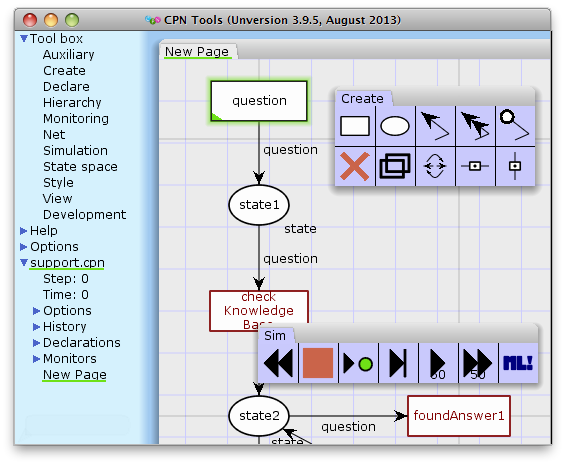
\includegraphics[scale=0.3]{images/cpntools.png}
	\caption{Capture d'écran : \brand{CPN Tools}}
	\label{fig.cpntools}
\end{figure}

\subparagraph{PNlib} \cite{pross2014object} est un outil de simulation orienté objet visant le cas particulier des processus biologiques.

La bibliothèque a été réalisé en \gls{modelica} et s'y intègre facilement.

\subparagraph{Snoopy} \cite{heiner2012snoopy} est un autre cadre logiciel à vocation unificatrice, permettant aussi l'utilisation de la couleur. Il supporte la hiérarchie.

Des outils d'analyse dynamique sont intégrés au logiciel.

Il a été appliqué aux réseaux biomoléculaires \cite{rohr2010snoopy}.

Une des particularités du logiciel est d'avoir plusieurs vues pour le même modèle, et d'aleterner facilement entre ces vues. Par exemple, il est possible d'avoir un modèle stochastique et un modèle continu pour le même réseau, qui partagent certaines propriétés.

\subsection{Applications récentes}
Il serait très dur d'établir un inventaire complet des utilisations des réseaux de Petri : comme pour les automates, les machines de Turing, ou encore le lambda-calcul, c'est un outil avec une très forte puissance d'expression, qui peut donc être utilisé dans une variété d'environnements différents, à des fins de modélisation.

Par exemple, à l'origine, C. A. Petri avait conçu les réseaux qui portent aujourd'hui son nom afin de modéliser des réactions chimiques. Ils sont maintenant très utilisés dans les modélisations de comportements biologiques \cite{koch2014petri}.

\subsubsection{Parallélisme}
Une des applications les plus courantes des réseaux de Petri est de simuler des systèmes répartis.

Un domaine annexe est celui de la parallélisation. Récemment, des progrès ont été fait dans la gestion de l'ordonnancement dans le cas d'applications s'exécutant en parallèle\cite{chen2014research}. Notamment, le système est modélisé à l'aide d'un réseau de Petri, et un algorithme génétique est utilisé pour y rechercher un chemin permettant un temps d'exécution minimal. 

\subsubsection{Application aux interfaces homme-système}
Les réseaux de Petri peuvent servir à modéliser toutes sortes de systèmes se basant sur une succession d'évènements.
 
Ils ont par exemple été utilisés pour la modélisation des interactions homme-système\cite{campos2014elementary}, avec différentes catégories d'évènements, comme le dépassement d'un seuil ou l'émission d'un signal, ce qui permet par la suite d'effectuer une analyse statique qui pourrait montrer des failles dans la conception du dit système.

\subsubsection{Application à des modèles cyber-physiques}
La \gls{cyberphysique} peut tirer un certain bénéfice des réseaux de Petri pour la simulation de son bon fonctionnement. En effet, elle consiste en différents éléments répartis et communiquants.

Des réseaux de Petri spatio-temporels ont été introduits\cite{zhang2014modeling} pour gérer les aspects de déplacements physique au cours du temps dans ce cas.

\subsubsection{Application aux jeux vidéos}
Les jeux vidéos peuvent parfois se présenter comme des processus scénarisés, que ce soit dans le temps, ou dans l'espace.
Une autre famille de réseaux spatio-temporels ont été introduits dans \cite{natkin2004new}, servant à prévoir et agir en fonction des déplacements des joueurs dans des niveaux de jeu.

Plus récemment, une classe de réseaux de Petri dédiée à des buts organisationnels, les \textit{WorkFlow nets}\cite{oliveira2011game}, ont été appliqués à la modélisation de jeu vidéo.
\section{Répartition}
La répartition (\textit{distribution}) est un second point important de ce stage. C'est un domaine qui est souvent très proche de la technique : le besoin d'utiliser des algorithmes répartis provient souvent de contraintes matérielles ou temporelles.

\subsection{Ouvrages de référence}
Plusieurs livres sont dédiés à des présentations générales du sujet, celui-ci étant étudié depuis plusieurs décénnies.

Au niveau des algorithmes, le livre de Nancy Lynch \cite{lynch1996distributed} présente les cas et problèmes les plus courants, en séparant les méthodes synchrones et asynchrones. 

Un autre ouvrage \cite{attiya2004distributed} met plus l'accent sur la simulation d'algorithmes distribués.

\subsection{Vérification}
La vérification des algorithmes distribués est une branche majeure qui nécessite des outils particuliers par rapport aux méthodes formelles usuelles, comme la \gls{logiquedehoare} telle qu'elle fut définie à l'origine par exemple.

Les outils de base sont la sécurité (\textit{safety}) et la vivacité (\textit{liveness}), telles qu'énoncées par Leslie Lamport \cite{lamport1977proving}.

De nombreux articles plus ou moins récents sur ce sujet sont référencés par un laboratoire de l'université de l'Illinois \cite{formaldistributed}.

Un des aspects particulièrement important dans le cas d'algorithme distribué est celui de la tolérance aux pannes. Par exemple, comment faire si un câble est débranché ? Et, plus précisément ici, comment vérifier qu'un algorithme donné sera tolérant aux pannes possibles ? 

Un exemple est donné \cite{mcmillan2014verification} pour le cas des algorithmes de consensus, qui introduit une logique de premier ordre particulière (nommée \textit{Consensus verification logic}).

Une autre approche utilisée est celle des algorithmes de transmission de messages \cite{jezequel2014message}, qui a été appliquée à la vérification de certains protocoles distribués, comme par exemple un protocole de \gls{mutex}.

\subsection{Développement}
Cette partie traitera des publications récentes ayant trait à l'implémentation des algorithmes de répartition.

Un ouvrage récent \cite{varela2013programming} fait le lien entre la théorie et la pratique, en présentant les méthodes les plus récentes pour écrire certains algorithmes. Un accent est mis sur la manière dont différents langages de programmation vont permettre plus ou moins simplement de réaliser différents paradigmes. Il tient aussi compte des avancées sur le \gls{calculambiant}, le \gls{picalcul}, et le \gls{joincalcul}.

\subsubsection{Modèles au fait des données (\textit{data-aware})}
Un algorithme opère toujours sur des données, néanmoins les opérations relatives à ces dernières (déplacement, envoi...) sont souvent considérées comme secondaires et comme quelque chose sur lesquelles l'auteur de l'algorithme distribué n'a pas de pouvoir.

Néanmoins, avec l'avènement du \gls{bigdata}, il est nécessaire de mieux prendre en compte cet aspect, parfois au niveau du système d'exploitation, ou encore des protocoles de routage utilisés \cite{baehni2004dependable} car les effets de bord deviennent trop volumineux.

Ainsi, des nouveaux paradigmes d'ordonnancement ont été proposés \cite{yildirim2012data, kosar2009paradigm}, ainsi que des méthodes pour optimiser le transfert de ces données.

\subsubsection{Routage}
Le routage est une problématique centrale des systèmes répartis, l'idéal étant de minimiser son temps.

Une méthode a été récemment proposée pour réduire ce temps en cas de forte charge sur les lignes, mais uniquement dans des cas de réseaux statiques \cite{jeon2014fully}.

% % % % Modularity in the design of robust distributed algorithms

De plus, il est intéressant de noter que des problèmes de routage comme la gestions des congestions peuvent s'appliquer à d'autres types de réseaux que les réseaux informatiques. Par exemple, des algorithmes ont été développés pour gérer en temps réel les problèmes des feux de circulation \cite{aoxue2014distributed}, en s'inspirant du concept de \gls{mutex} et en utilisant des capteurs embarqués sur chaque véhicule.

\subsubsection{Réseaux sans-fil}
Les réseaux sans-fil sont désormais omniprésents, et offrent de nouvelles opportunités d'optimisation qui leur sont propres.

Par exemple, il a été montré dans \cite{hosseinabadi2014exploiting} que les paquets entendus par un client mais qui ne lui étaient pas directement destinés (\textit{overheard packets}) pouvaient être utilisés pour améliorer la performance du réseau (et notamment les temps d'attentes dûs aux collisions), à l'aide d'algorithmes spécifiques.

Un outil, \brand{FlockLab} \cite{lim2013flocklab} a été conçu spécifiquement pour la vérification et l'analyse de réseaux sans-fil embarqués. Il permet le débogage, et l'étude des timings à une précision proche de la microseconde en utilisant les protocoles généralement utilisés sur l'embarqué, comme \ac{GPIO}.  

\section{Synchronisation}
Les problèmes de synchronisation sont généralement vus comme une sous-partie des problèmes inhérents aux systèmes embarqués. Néanmoins, dans ce sujet, c'est une des partie les plus importantes et pertinentes, en raison de ce qui a été expliqué en \cref{section.pbRepart}.

La synchronisation implique toujours un concept d'horloges. Deux familles sont présentées : les horloges logiques, qui servent à ordonner les éléments entre eux, et les horloges physiques, qui servent de référence absolue.

\subsection{Synchronisation logique}
\subsubsection{Origines : les horloges de Lamport}
Le premier système d'horloge logique est celui conçu par Leslie Lamport, récipiendaire du prestigieux \textit{Turing Award 2013}.

Il a notamment conçu les horloges et horodatages (\textit{timestamps})~\cite{lamport1978time} qui portent son nom, et qui expriment la notion de "arrivé-avant".
\subsubsection{Horloges vectorielles}
Les horloges vectorielles (\textit{vector clocks}) sont une amélioration au dessus du concept des horloges de Lamport.

Néanmoins, plutôt que de ne faire garder que leur état logique aux nœuds, on leur fait garder l'état de tous les nœuds dont ils ont reçu des messages dans un vecteur\cite{fidge1988timestamps}. Lorsqu'un nœud envoie un message à un autre, ce dernier se met à jour avec les horodatages maximaux contenus dans le vecteur qui est envoyé.

Le problème des horloges vectorielles est la croissance de la taille du vecteur dans un système contenant beaucoup de nœuds.

\paragraph{Horloges plausibles}
Une méthode pour régler le problème de taille de vecteur a été proposée dans \cite{torres1999plausible}. Cela améliore l'efficacité dans le cas de grands réseaux, néanmoins il arrive que des évènements pouvant se dérouler en parallèle soient réorganisés pour se dérouler séquentiellement.

\subsection{Synchronisation physique}
Comme i-score est un logiciel permettant de manipuler le temps, il nécessite de travailler avec une horloge physique. Le problème principal des systèmes distribués se basant sur une horloge est de s'assurer que tous les nœuds ont la même heure.

\subsubsection{Algorithmes couramment utilisés}
En pratique, il existe deux méthodes couramment utilisées pour garantir une synchronisation des horloges entre machines.

\subparagraph{NTP} (\textit{Network Time Protocol}) est la méthode couramment utilisée sur Internet pour synchroniser l'heure des machines.

Elle emploie une structure en arbres avec plusieurs niveaux, chacun communiquant uniquement avec ses niveaux supérieurs et inférieurs.

Elle permet une synchronisation de l'ordre de quelques millisecondes seulement à l'échelle de l'internet \cite{mills1991internet}.
\subparagraph{PTP} (\textit{Precision Time Protocol}) est une méthode qui a été développée après \brand{NTP}, et qui est optimisée pour les réseaux locaux requérant une plus grande précision que celle que peut offrir \brand{PTP}.

Elle permet une synchronisation de l'ordre de $\num{1}\si{\micro\second}$ \cite{peng2009research, scheiterer2009synchronization}. La viabilité des algorithmes utilisés par \ac{PTP} sur systèmes \brand{Android} a été démontrée dans \cite{hsu2012measurement}.

En revanche, le nombre de paquets transmis est plus élevé que dans le cas de \ac{NTP}, ce qi peut poser problème en cas de charge élevée sur le réseau.
\subsubsection{Autres approches}
Une méthode dédiée aux réseaux ayant une possibilité de \textit{broadcast}, c'est-à-dire de transmission à tous les clients, a été présentée dans \cite{elson2002fine}. Elle offre de meilleures performances que \ac{NTP}, et possède comme différence avec les méthodes couramment utilisées la non-transmission de timestamps : les horloges sont déduites à partir des temps d'arrivée des messages.

D'autres approches ont essayé d'utiliser d'autres couches que les couches applicatives pour synchroniser les horloges. C'est le cas de \cite{abari2014one} : une approche dédiée aux réseaux sans-fil, qui modifie directement les couches physiques pour qu'elles se synchronisent entre elles automatiquement sur une horloge unique, présente dans le signal sans-fil, plutôt que sur leurs horloges internes généralement gérées par des quartz dont la fréquence peut être légèrement variable.

Enfin, des recherches ont été faites pour gérer les cas de réseaux peu fiables et possédant de grandes latences. Un mécanisme pour gérer les synchronisations par transmission acoustique dans des milieux marins est présenté dans \cite{syed2006time}. Ces cas ont des contraintes très importantes en terme de débits et de pertes de bits, ce qui force l'utilisation d'algorithmes dédiés, qui prennent notamment en compte le décalage d'horloges (\textit{clock skew}) qui peut être particulièrement important.
\subsection{Estimation de la latence}
\label{section:latence}
Il est critique dans de nombreuses applications collaboratives et réparties de pouvoir estimer la latence entre les différentes machines, et ce de la manière la plus précise possible. Cela peut s'appliquer dans le cas de réseaux locaux à haute vitesse, ou bien de l'internet.

L'algorithme le plus simple consiste en un message de type ping/pong entre deux machines, mais la précision est très faible, et il n'est pas possible de connaître la latence dans une seule direction.

Des méthodes plus perfectionnées peuvent par exemple faire appel à une machine tierce et des points de repères présents sur le réseau : \cite{banerjee2012network}, ou encore à des comportements entièrement pair-à-pair \cite{im2000method} qui fonctionnent sur des versions avancées de l'algorithme naïf présenté au paragraphe précédent. 
Une autre approche, purement logicielle, nommée \brand{King} \cite{gummadi2002king}, fait appel à des requêtes \ac{DNS} récursives. Ainsi, cette méthode se destine principalement à une utilisation sur internet.

\section{Projet OSSIA et partitions interactives}
Le projet \ac{OSSIA} utilise les acquis du projet \brand{Virage} \cite{baltazar2009virage} qui l'a précédé, ainsi que ceux de différents formalismes de partitions interactives. Il est aussi en interaction avec le projet \brand{INÉDIT} \cite{fober2013caracterisation} qui vise à rendre interopérable différents outils de création musicale et de composition.

\subsection{Partitions interactives}
\subsubsection{Origines : Boxes}
Les premières recherches ont porté sur une méthode de combiner des structures fréquentielles entre elles afin de composer un morceau. Ces travaux, réalisés aux alentours de l'an $\num{2000}$ ont posé les bases des développements actuels, en introduisant les concepts de contraintes, de boites temporelles et de hiérarchisation dans le même logiciel \cite{beurive2000logiciel}, nommé \brand{Boxes}.
\subsubsection{Premières méthodes}
Les partitions interactives ont été à l'origine conçues pour offrir un formalisme, et donc des possibilités de provabilité et de vérification, au cas de la composition musicale. 
L'idée originale a été de concevoir les partitions interactives comme un ensemble d'objets temporels rattachés à des relations d'Allen \cite{allen1983maintaining}, qui sont une forme de contraintes logiques adaptées aux évènements temporels. Les objets temporels peuvent contenir un processus et une contrainte locale \cite{allombert2007system}, et peuvent faire partie de différentes classes prédéfinies afin d'aider le compositeur. 

L'interactivité provient du fait que des évènements peuvent être déclenchés en temps-réel, sur scène, par un compositeur ou musicien, tout en maintenant une logique qui aura été écrite au préalable. Par exemple, la lecture d'une vidéo $V$ suit automatiquement la lecture d'un son $S$, lui-même déclenché lors de l'activation d'un capteur extérieur. 

Une des problématiques principales est donc de maintenir les contraintes entre objets temporels, tout en permettant l'interactivité.

Plusieurs méthode ont été étudiées pour répondre à ce problème :
\begin{itemize}
\item Une méthode par contraintes concurrentes, inspirée de \ac{NTCC} \cite{allombert2006concurrent}.
\item Une méthode par réseaux de Petri \cite{allombert2007system, allombert2009aspects}.
\end{itemize}

Ces méthodes ont été implémentées, avec de multiples extensions (présentées en détail dans \cite{mauricio2012structured} en section 3.2) dans les différents logiciels présentés en \cref{figheritageIScore}.

\subsection{Précision des formalismes}
Un des problèmes dans les méthodes présentées par Antoine Allombert est l'absence de modèle réunissant branchements et relations temporelles.

Une solution possible, nommée \textit{Time Conditional-Branching Scores}, est avancée par Mauricio Toro dans sa thèse \cite{mauricio2012structured}.

\subsection{Problématique du traitement de signal}
Bien qu'à l'origine, le lien entre partitions interactives et traitement du signal était fort, notamment dans le logiciel \brand{Boxes}, les recherches plus récentes ont porté majoritairement sur un formalisme uniquement scénaristique, sans réelle préoccupation de ce qui était scénarisé.

Un des problèmes principaux rencontrés est la gestion du temps : en effet, les cartes sons ont leur propre fréquence d'horloge, qui est généralement de $\num{44100}\si{\hertz}$, et fonctionnent par buffers, ce qui n'est pas toujours le cas des logiciels implémentant les différents formalismes de partitions interactives.

Néanmoins, des approches ont été menées en parallèle pour essayer de relier les deux. Mauricio Toro présente dans sa thèse une méthode pour inclure des processus \ac{FAUST} dans une partition interactive \cite[chapitre 8]{mauricio2012structured}.
Cette approche est continuée par Florent Berthaut avec le travail mené sur \brand{libLAScore}, une bibliothèque intégrant \brand{LibAudiostream} (qui implémente \ac{FAUST}), et \brand{libIscore} \cite{desaintecatherine2014interactive}.

Actuellement, un autre modèle entièrement basé sur la sémantique des réseaux de Petri, qui fonctionne par envoi de jetons correspondant aux paquets de donnée, est en cours de développement par Jaime Arias \cite{arias2014modelling}.

\subsection{Développement dans OSSIA}
Le projet \ac{OSSIA} se place à un niveau plus abstrait que les différents formalismes de partitions interactives.

